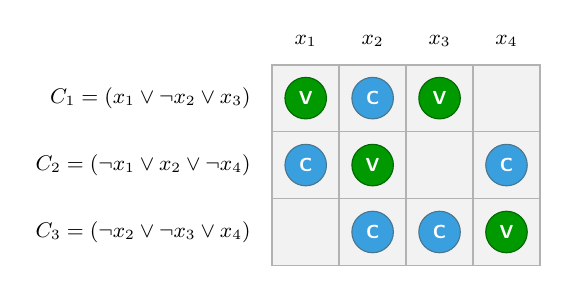
\begin{tikzpicture}[
    scale=0.85,
    transform shape,
    celda/.style={draw=gray!60, fill=gray!10, line width=0.6pt},
    verde/.style={circle, fill=green!60!black, draw=green!40!black, minimum size=0.62cm, inner sep=0pt, font=\footnotesize\sffamily\bfseries\color{white}},
    celeste/.style={circle, fill=cyan!75!blue!80, draw=cyan!50!black, minimum size=0.62cm, inner sep=0pt, font=\footnotesize\sffamily\bfseries\color{white}}
]
    \draw[celda] (0,0) rectangle (4,3);
    \draw[celda] (0,0) grid (4,3);

    % Encabezados de columnas (Variables)
    \node[font=\small\bfseries] at (0.5, 3.35) {$x_1$};
    \node[font=\small\bfseries] at (1.5, 3.35) {$x_2$};
    \node[font=\small\bfseries] at (2.5, 3.35) {$x_3$};
    \node[font=\small\bfseries] at (3.5, 3.35) {$x_4$};

    % Etiquetas de filas (Cláusulas)
    \node[anchor=east, font=\small] at (-0.2, 2.5) {$C_1 = (x_1 \lor \neg x_2 \lor x_3)$};
    \node[anchor=east, font=\small] at (-0.2, 1.5) {$C_2 = (\neg x_1 \lor x_2 \lor \neg x_4)$};
    \node[anchor=east, font=\small] at (-0.2, 0.5) {$C_3 = (\neg x_2 \lor \neg x_3 \lor x_4)$};

    % Piedras Fila 1
    \node[verde] at (0.5, 2.5) {V};
    \node[celeste] at (1.5, 2.5) {C};
    \node[verde] at (2.5, 2.5) {V};

    % Piedras Fila 2
    \node[celeste] at (0.5, 1.5) {C};
    \node[verde] at (1.5, 1.5) {V};
    \node[celeste] at (3.5, 1.5) {C};

    % Piedras Fila 3
    \node[celeste] at (1.5, 0.5) {C};
    \node[celeste] at (2.5, 0.5) {C};
    \node[verde] at (3.5, 0.5) {V};
\end{tikzpicture}

